\documentclass{article}
\usepackage[utf8]{inputenc}
\usepackage{graphicx}
\usepackage{amsmath}
\graphicspath{ {./images/} }
\setlength{\parindent}{0em}


\title{QLSC 612 Assignment}
\author{Vladimir Grouza and Co.}
\date{31 May 2020}

\begin{document}

\maketitle

\textbf{Introduction}\\*

Previously, Willerman et al (1991) investigated a correlation between brain size and full scale intelligence quotient (FSIQ) in a population of psychology students (n = 40). Their analysis showed a positive linear correlation in the male population ($\rho$ = 0.50, p = 0.03, n = 20) but not in the female population ($\rho$ = 0.32, p = 0.16, n = 20), implying a direct relationship between brain volume and intelligence. In this work, we attempt to extend the relationship between intelligence and other physical metrics. In particular, we hypothesize that since an individual is smarter and larger, they must also be faster. We explore this relationship by measuring the subject reaction time in a button-press task following a stimulus. Since the acceleration of a limb is the second derivative of its position, we further hypothesize that intelligence and reaction time exhibit a non-linear correlation. \\*

\textbf{Methods} \\*

In order to maintain maximum reproducibility, we recruited every single individual used in Willerman's 1991 study. Subjects were presented with a light flash stimulus and asked to depress a button as soon as they perceived it. The reaction time was then correlated with FSIQ using Spearman's rank correlation coefficient. Finally, in order to account for subject mental state and fatigue, we then repeated the study a full year later.\\*

\textbf{Results}\\*

In the first iteration, the reaction time across all individuals was measured to be $98.2 \pm 10.0$ milliseconds (n = 40). Reaction time and FSIQ exhibited a statistically significant correlation ($\rho = 0.34$, p = 0.03). The trivially obvious relation is elegantly visualized in Figure 1. In the second iteration, the reaction times were $100.2 \pm 10.0$ milliseconds again, demonstrating how reproducible our study is. Inconceivably however, the correlation was somewhat lower and only almost statistically significant ($\rho = 0.27$, p = 0.09). \\*

\textbf{Discussion}\\*

We have provided very convincing proof that speed and intelligence are obviously related. While the second iteration was only almost statistically significant for correlation between reaction time and FSIQ, we hypothesize that this is because many of the subjects were beginning to show signs of aging and dementia by the time of conduction of the second study. We have graciously provided all of our analysis and data files online, and leave it to the reader to remove aberrant subjects to show push our p-value below to 0.05. 



\begin{figure}[h]
    \centering
    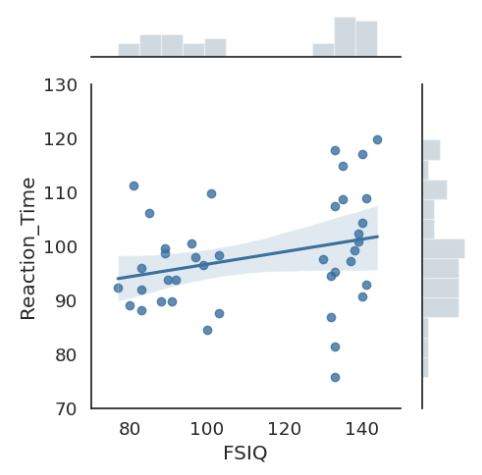
\includegraphics[scale = 0.65]{figure.png}
    \caption{\small{captions}}
\end{figure}

\textbf{References}\\*

[1] Lee Willerman, Robert Schultz, J. Neal Rutledge, and Erin D. Bigler. In vivo brain size and intelligence. \emph{Intelligence} 1991; 15(2):223-228. 



\end{document}
